% This is LLNCS.DEM the demonstration file of
% the LaTeX macro package from Springer-Verlag
% for Lecture Notes in Computer Science,
% version 2.4 for LaTeX2e as of 16. April 2010
%
\documentclass{llncs}
\usepackage{graphicx}
%
\begin{document}
%
\title{Mobile Application Development with MELON}
%
\author{Justin Collins \and Rajive Bagrodia}
%
%%%% list of authors for the TOC (use if author list has to be modified)
\tocauthor{Justin Collins, Rajive Bagrodia}
%
\institute{University of California Los Angeles, Los Angeles CA, USA,\\
\email{\{collins, rajive\}@cs.ucla.edu}}

\maketitle

\begin{abstract}
Developing distributed applications for mobile ad hoc network continues to be challenging due to the dynamic and unpredictable nature of MANETs. MELON is a general purpose coordination language designed to provide flexible communication patterns for MANET applications while remaining lightweight. Based on a distributed shared message store, MELON abstracts network communication to an asynchronous exchange of persistent messages. MELON simplifies application development by supporting read-only and remove-only messages, bulk message retrieval, and per-host ordering of messages. In this paper, we review the MELON programming model, demonstrate its utility for writing MANET applications, and quantitatively compare it to traditional distributed computing paradigms in a MANET context.
\end{abstract}
%

\section{Introduction}

Tiny, powerful personal computers are quickly becoming ubiquitious. In the United States, 91\% of adults have cell phones, and 56\% of those are smartphones\cite{cellphones}. Among teens, 78\% have a cell phone, of which 37\% are a smartphone\cite{teenphones}. Add smartphones to the proliferation of tablets and laptops and the ability for consumers to form mobile ad hoc networks (MANETs) is quickly becoming possible. However, applications designed for these networks remain in short supply. Developing MANET applications face a number of challenges, with the primary difficulty being the unpredictably dynamic infrastructureless wireless network itself. Unlike wired networks, failures in MANETs are commonplace instead of exceptional. Nodes may join and leave the network at any time and the network topology is in constant flux. Networked applications must be aware of and handle the challenging nature of MANETs to be useful.

Several language, middleware, and library solutions to dealing with MANET communication have been proposed to assist in developing MANET applications. The majority of these proposals are based on traditional distributed computing paradigms\cite{mine}. Of these, publish/subscribe, remote procedure calls, and tuple spaces are commonly used. However, these communication paradigms were originally designed for stable, wired networks or even interprocedural communication on a single machine. While they have been adapted to MANETs, their original designs are limiting and not well-suited to the MANET environment\cite{collins2010quantitative}.

To address the need for a communication paradigm designed specifically to operate in MANETs, we have proposed a new coordination language called MELON\cite{melon}. MELON provides a flexible, general-purpose communication abstraction which may be completely distributed. In addition to basic message exchange, MELON also implements bulk message retrieval, provides basic message access control, enforces per-host ordering of messages, and supports message streams.

In this paper we describe the MELON paradigm, compare implementing a shared whiteboard application with publish/subscribe, RPC, tuple spaces, and MELON, and finally compare the performance of each whiteboard implementation. We demonstrate MELON is well-suited for developing MANET applications, and while slower than publish/subscribe and RPC, it is the only paradigm to deliver 100\% of sent messages. MELON also delivered whiteboard messages with 95\% less latency and 60\% more in-order messages when compared to tuple spaces.

In Section \ref{sec:design} we review the design of MELON and operations it provides, then discuss the implementation in Section \ref{sec:implementation}. We compare shared whiteboard implemented with different paradigms in Section \ref{sec:wb} and then measure performance of each paradigm in Section \ref{sec:comparison}. Section \ref{sec:relatedwork} describes related work and finally our conclusions are presented in Section \ref{sec:conclusions}.

\section{MELON Design}\label{sec:design}

The MELON communication paradigm borrows the idea of a distributed shared message store from Linda\cite{linda} and LIME\cite{lime}. The concept of tuple spaces - shared collections of messages which may be manipulated by many processes - fits well in a MANET context. To send a message, a process stores it in a globally shared memory ``space". Messages are retrieved by matching them against desired templates. This decoupling between sending and receiving is beneficial in a MANET context, where maintaining connections between hosts can be challenging. With tuple spaces, disconnections no longer cause disruptions to communications, only delays in retrieving messages.

However, aside from the shared message store, MELON departs significantly from typical tuple spaces in its operations and semantics. In a tuple space, any message may be read or removed by any process, and any matching message may be retrieved in any order. For non-destructive reads, the same tuple may be returned multiple times. In contrast, MELON divides the messages into two pools: a remove-only pool, and a read-only pool. Remove-only messages can only be retrieved once and must be removed when retrieved. Read-only messages may never be explicitly removed, they can only be copied from the message store. Messages are returned in a per-host ordering, although which host returns a matching message remains nondeterministic.

Given the prevalence of private messages in current mobile applications (e.g., SMS, instant messaging, direct messaging in social applications), one further option for messages is to make them private. A take-only message may be given an addressee, which is the only process permitted to read the message.

MELON contains some additional minor differences from tuple spaces. First, messages are not required by the paradigm to be tuples, but may be implemented as any structure, given they can be matched by a template (for example, messages could be unordered tuples with named values instead). Secondly, considering the storage limitations of mobile devices, MELON explicitly limits the space available on a host for storing messages. As a result, messages may be automatically garbage collected. A last deviation from tuple spaces is the removal of strict semantics for returning messages. In tuple spaces, the semantics stipulate that if a matching message exists, it must be returned for a retrieval operation. In the reality of MANETs, this semantic cannot be met, so in MELON all retrieval operations are limited to best-effort.

These differences were introduced in MELON to both relieve the application developer of certain responsibilities and to allow the paradigm to operate well in a MANET. For example, read-only messages prevent a badly-behaved process from removing important messages meant to be read by many processes, and per-host ordering is especially convenient in applications such as news feeds or streaming video, where most messages are generated by a single host and the ordering is important. MELON is also deliberately designed to avoid any global state and allow for a completely distributed implementation.

\subsection{MELON Operations}\label{melon}

Processes in MELON communicate by storing messages to a distributed shared message store and retrieving the messages based on templates. In this paper, we assume messages consist of an ordered list of typed values. However, as noted above, nothing in the paradigm itself limits how messages might be constructed,  A message template is similar to a message, except it may contain both values and types. For example, a message containing \texttt{[1, "hello"]} could be matched by a template containing \texttt{[1, String]} or \texttt{[Integer, "hello"]} or \texttt{[Integer, String]}. A type will also match any subtypes.

Operations are split into read-only (\textbf{write}/\textbf{read}/\textbf{read\_all}) and take-only (\textbf{store}/\textbf{take}/\textbf{take\_all}) operations. Each operation is represented here as a separate function call. \textbf{store} and \textbf{write} operations have return null values and return as soon as the saved message is available in the message store (essentially immediately). \textbf{take} and \textbf{read} operations block by default until a matching message is returned, but may be set to non-blocking on a per-call basis. If a non-blocking call finds no matching messages, it returns an empty set.

\begin{table}
\centering
\begin{tabular}{|c|c|c|}
\hline
\textbf{Operation} & \textbf{Return Type} & \textbf{Action} \\ \hline
\textbf{store}(\textit{message}, \textit{[address]}) & \textit{null} & Store removable message \\ \hline
\textbf{write}(\textit{message}) & \textit{null} & Store read-only message \\ \hline
\textbf{take}(\textit{template}, \textit{[block = true]}) & \textit{message} or \textit{null} & Remove and return message \\ \hline
\textbf{read}(\textit{template}, \textit{[block = true]}) & \textit{message} or \textit{null} & Copy and return read-only message \\ \hline
\textbf{take\_all}(\textit{template}, \textit{[block = true]}) & \textit{array} & Bulk remove messages \\ \hline
\textbf{read\_all}(\textit{template}, \textit{[block = true]}) & \textit{array} & Bulk copy read-only messages \\ \hline
\end{tabular}
\caption{MELON Operations}
\end{table}

When called, \textbf{store} saves a copy of the message in the message store. Messages saved with \textbf{store} may only be retrieved with a \textbf{take} or \textbf{take\_all} operation. If an address is provided, then only the host with a matching identity can remove the message.

The \textbf{write} operation also stores a single message in the message store, but the message may only be copied from the storage space with a \textbf{read} operation, never explicitly removed. Messages written with the \textbf{write} operation may be automatically garbage collected.

A \textbf{take} operation requires a message template as the first argument and an optional boolean for the second argument. The message template is matched against available messages in the message store which were added with a \textbf{store} operation. If a matching message is found, it will be removed from the message store and returned. Once a message has been returned by a \textbf{take} operation, it may not be returned by a subsequent operation in any process.

The \textbf{read} operation will only return messages stored with a \textbf{write} operation which have not already been read by the current process. If a message matching the given message template is available, it will be copied and returned, but not removed from the message store. Once a message has been returned to a process, the message is considered to have been read by that process and will not be returned by any subsequent \textbf{read} or \textbf{read\_all} operations in that process. A message may be \textbf{read} by any number of processes, but only once per process.

\begin{table}
\centering
\caption{Read from multiple processes}
\begin{tabular}{|c|c|c|} \hline
\textbf{Process A} & \textbf{Process B} & \textbf{Process C} \\ \hline
\texttt{write([1, "hello"])} & \texttt{m = read([Integer, String])} & \texttt{m = read([Integer, String])} \\ \hline
\end{tabular}
\label{fig:readprocesses}
\end{table}

Table \ref{fig:readprocesses} illustrates one process writing a single message containing the integer \texttt{1} and the string \texttt{"hello"}. Processes B and C each perform a \textbf{read} operation with the template which matches the message stored by process A. Since \textbf{read} does not modify the storage space, the value of \textit{m} for both process B and C will be a copy of the message \texttt{[1, "hello"]} from process A.

The \textbf{take\_all} and \textbf{read\_all} operations are used to retrieve a group of matching messages instead of a single message. Otherwise, the semantics match \textbf{take} and \textbf{read}: \textbf{take\_all} can only remove messages from \textbf{store} operations, and \textbf{read\_all} only returns unread messages from \textbf{write} operations.

\begin{table}
\centering
\caption{News server and reader}
\begin{tabular}{|c|c|} \hline
\textbf{News Server} & \textbf{News Reader} \\ \hline
\begin{minipage}{2.45in}
\begin{verbatim}

function report(category, headline) {
   write([category, headline])
} 
\end{verbatim}
\end{minipage}
&
\begin{minipage}{2.5in}
\begin{verbatim}


function fetch(category) {
   return read_all([category, String])
}
\end{verbatim}
\end{minipage}
\\ \hline
\end{tabular}
\label{fig:newsreader}
\end{table}

Table \ref{fig:newsreader} demonstrates a use of \textbf{read\_all}. One or more processes generate news messages containing a news category and headline. To ensure all interested parties can read the news, the server uses \textbf{write} to disallow a reader from removing a news item and preventing other readers from reading it. Any number of processes can consume the news as readers. The \texttt{fetch} method in Table \ref{fig:readprocesses} uses \textbf{read\_all} to return all news items in a given category. Repeated calls to \texttt{fetch} will only return news items not previously seen.

By default, all retrieval operations will block the application until at least one matching message is found. The operations can also be performed in nonblocking mode, in which case \textbf{take} and \textbf{read} return null when no matching message is found, while \textbf{take\_all} and \textbf{read\_all} return empty collections.
   
\subsection{MELON Implementation}\label{sec:implementation}

\begin{figure}
\centering
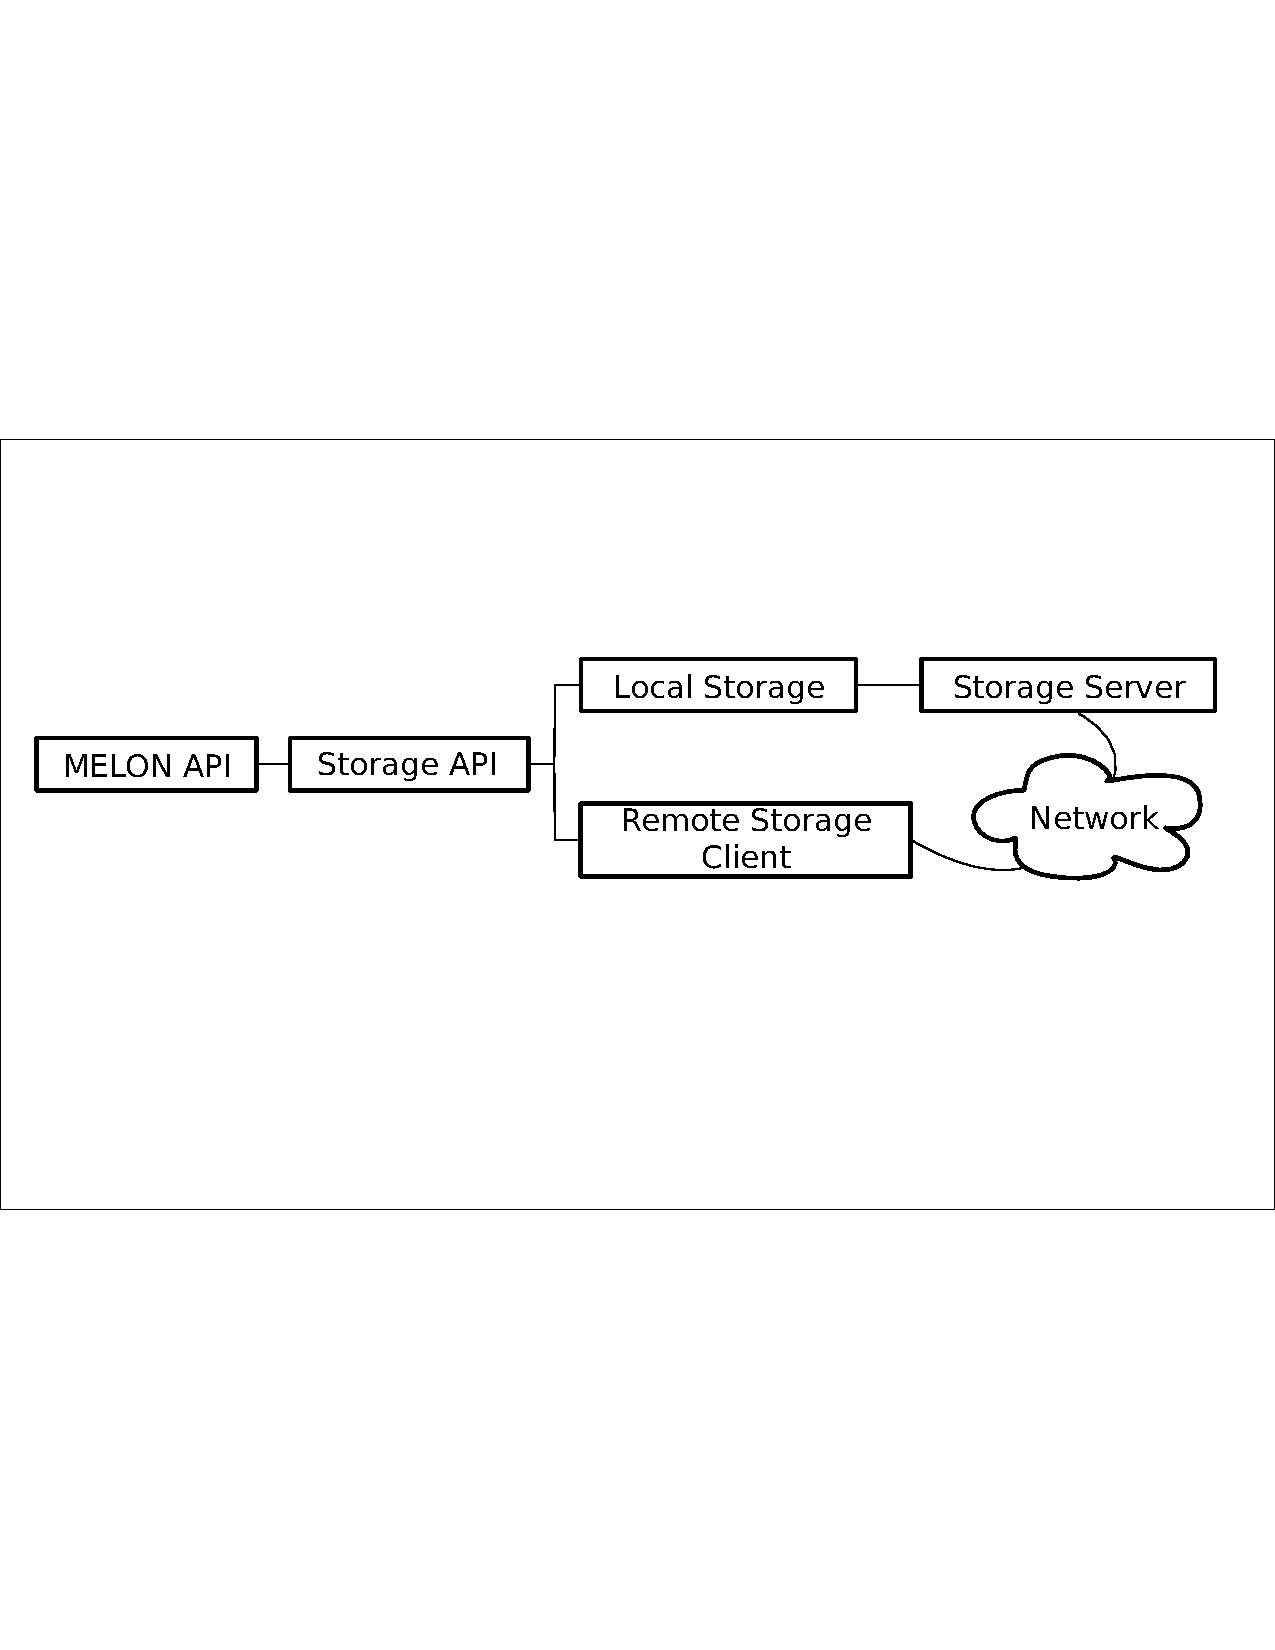
\includegraphics[scale = .50, clip, trim = 10px 350px 10px 312px]{figures/paradigm_arch.pdf}
\caption{Paradigm Architecture}
\label{fig:architecture}
\end{figure}

We developed a prototype implementation of MELON to validate our design and obtain empirical performance data. The architecture illustrated in Figure \ref{fig:architecture} is split into five parts. The MELON API is the only interface exposed to the application and provides the six operations described above. The MELON API interacts with the distributed message storage through the storage API, which provides the same interface for both local and remote storage. The storage server proves a network interface to a local storage space and accepts connections made through the remote storage stub.

Local storage is implemented as two dynamic arrays, one for \textbf{write}/\textbf{read} messages and the other for \textbf{store}/\textbf{take} messages. For atomic updates, the \textbf{write}/\textbf{read} array uses a readers/writer lock to allow multiple \textbf{read} operations to access the array concurrently, but locks the array for \textbf{write} operations. The \textbf{store}/\textbf{take} array does not permit concurrent operations, as \textbf{store} and \textbf{take} modify the store. The two arrays may be accessed and modified independently.

Network communication is handled by ZeroMQ\cite{hintjens2013zeromq}, a high performance networking library. For the prototype, the networking was intentionally kept simple. For example, a \textbf{read} request queries remote hosts in random order and stops when a matching result is returned. This could possibly be improved using multicast, but it would complicate the implementation by requiring the client to handle multiple asynchronous responses, select one, request the actual message, and handle failure scenarios if the matching message cannot be returned. We traded potential performance gains for simplicity. 

For \textbf{read} and \textbf{read\_all} operations, it is necessary to track which messages have been read. Each process maintains its own list of read messages, which it sends with each \textbf{read} request. We use a compact sparse bit set to track and transfer this information efficiently.

\section{Shared Whiteboard Example}\label{sec:wb}

A shared whiteboard is a digital document which may be edited and viewed by multiple users concurrently and is commonly proposed as an example of an application well-suited to MANETs\cite{wb5}\cite{wb6}. It is distributed, real-time, and allows participants to share information. It also presents some interesting characteristics. Since many participants may be updating the whiteboard, ordering of changes is very important to maintain a consistent document. It is also important that changes be propagated quickly so that each user is working with the latest document.

We have implemented a shared whiteboard in MELON, publish/subscribe, RPC, and tuple spaces using JRuby (a Java implementation of the Ruby language) in order to compare their features and performance.
Each version shares common code related to the actual whiteboard itself, which is implemented in the Whiteboard class.
Changes to the shared whiteboard are encapsulated in a Figure object. Each version implements an \texttt{add\_local\_figure} method which is called when the user modifies the shared whiteboard.
The MELON and tuple space versions also implement an \texttt{add\_remote\_figures} method which is used to retrieve updates from remote nodes.

\subsection{Publish/Subscribe}

The publish/subscribe paradigm divides processes into publishers and subscribers. In topic-based publish/subscribe, publishers simply publish messages tagged with a topic identifier. Subscribers receive the messages by subscribing to one or more topics and specifying a callback to handle the publications asynchronously and separately from the main process thread. It is also possible to handle multiple incoming publications concurrently. Publish/subscribe does not guarantee any ordering of publications nor does it specify how to deliver messages if the subscribers is not available at the time of publication. In distributed publish/subscribe such as MANETs, it is generally not expected that publishers would persist and deliver messages at a later time\cite{psfaces}.

The publish/subscribe whiteboard in Table \ref{fig:pswb} sets up a subscription to the ``whiteboard" topic and a callback to add remotely published figures to the whiteboard. This allows the whiteboard to receive updates at any time in a separate thread, which is precisely what would be desired. To output a new figure, the whiteboard simply publishes the figure to the ``whiteboard" topic.

\begin{table}
\centering
\begin{tabular}{c c}
\begin{minipage}{2.75in}
\begin{verbatim}
require "ps"
require "whiteboard"

class PSWhiteboard < Whiteboard
  def initialize
    @ps = PS.new
    
    @ps.subscribe "whiteboard" do |figure|
      add_figure figure
    end
  end

  def add_local_figure figure
    @ps.publish "whiteboard", figure
  end
end
\end{verbatim}
\caption{Publish/Subscribe Whiteboard}
\end{minipage}\label{fig:pswb}
&
\begin{minipage}{2.5in}
\begin{verbatim}
require "rpc"
require "whiteboard"

class RPCWhiteboard < Whiteboard
  def initialize
    @rpc = RPC.new
    @rpc.export self
  end

  def add_local_figure figure
    wbs = @rpc.find_all "RPCWhiteboard"
    wbs.add_figure figure
  end
end


\end{verbatim}
\caption{RPC Whiteboard}
\end{minipage}\label{fig:rpcwb}
\end{tabular}
\end{table}


\subsection{RPC}

Remote procedure calls (RPC) is a distributed programming paradigm which disguises remote communication as local method calls. A host can ``export" an object to be accessed remotely. Remote hosts discover these remote objects by name and then invoke methods on them. Arguments may be passed to the remote method and the return value of the method is returned to the local process. A variation of this used in our example is group RPC, which allows us to invoke the same method with the same arguments on all known remote objects of the requested type. These calls are performed asynchronously. Typically the return values would be handled by a callback, but this functionality is not used in our example.

A shared whiteboard implementation using RPC is listed in Table \ref{fig:rpcwb}. When the whiteboard is initialized, it is also exported as a remote object. This allows other hosts to remotely invoke the \texttt{add\_figure}. Like publish/subscribe, this allows the whiteboard to accept remote figures asynchronously from the main process thread and is a natural feature of RPC. Distribution of remote figures is performed by first finding all remote instances of \texttt{RPCWhiteboard}, then invoking the \texttt{add\_figure} method (defined on the parent class) directly, passing in the new figure as an argument. Since the group RPC is asynchronous, it is possible that a call might complete before a prior call.

\subsection{Tuple Spaces}

Tuple spaces operate on a distributed shared memory space full of ordered tuples. Tuples may be output using the \textbf{out} operation, then retrieved using \textit{rd}, which copies the tuple, or \textit{in}, which removes the tuple from the tuple space based on matching templates. If multiple tuples match a template, one of the matching tuples is chosen nondeterministically to be returned.

Table \ref{fig:tswb} shows the tuple space version, which is very similar to MELON. To send an update, it outputs a tuple containing just the new figure. Unlike MELON, a misbehaving or misconfigured client could remove the messages from the tuple space, disrupting the shared whiteboard communication. Retrieval of remote messages uses a \textbf{bulk\_rd} operation to read all messages containing a figure. To continuously retrieve messages asynchronously, this method can be called inside a loop in a separate thread. Once a group of figures is retrieved, each individual figure is added to the local whiteboard. 

Tuple spaces suffer from the multiple read problem\cite{mrdp}: repeated nondestructive read operations (\textbf{rd}) may return any matching tuple, including the same tuple. As discussed in \cite{mrdp}, one solution is to use a mutex tuple to gain exclusive access to the tuple space, remove all the desired tuples using \textbf{in}, then replace all the tuples and release the mutex. However, this approach removes all concurrent access and is dangerous in a MANET where the node holding the mutex may disappear. Another solution is to use a counter in each tuple, then read tuple 0, then tuple 1, and so on. Then each process can request tuples by the counter value. However, if multiple processes are producing tuples they must coordinate to produce consistent counters, essentially resulting in a producer-side mutex.

Finally, \cite{mrdp} proposes a \textbf{copy-collect} operation, which copies all matching tuples. We have implemented this as the \textbf{bulk\_rd} operation as used in Table \ref{fig:tswb}. However, this does not solve what might be termed the ``multiple multiple read problem": since our tuple space is not static, reading all matching tuples once is not sufficient. We need to be able to perform multiple \textbf{bulk\_rd}s to get all figures added to the whiteboard. Without \textit{a prior} knowledge of remote hosts in the system, the only option which allows concurrent access to the tuple space is to read \textit{all} matching tuples. Naturally, this is quite expensive as the number of tuples grows. 

\begin{table}
\centering
\begin{tabular}{c c}
\begin{minipage}{2.75in}
\begin{verbatim}
require "melon"
require "whiteboard"

class MelonWhiteboard < Whiteboard
  def initialize
    @melon = Melon.new
  end
  
  def add_local_figure figure
    @melon.write [Figure]
  end

  def add_remote_figures
    figures = @melon.read_all [Figure]

    figures.each do |figure|
      add_figure figure[0]
    end
  end
end
\end{verbatim}
\caption{MELON Whiteboard}
\end{minipage}\label{fig:mwb}
&
\begin{minipage}{2.5in}
\begin{verbatim}
require "tuplespace"
require "whiteboard"

class TSWhiteboard < Whiteboard
  def initialize
    @ts = Tuplespace.new
  end

  def add_local_figure figure
    @ts.out [Figure]
  end

  def add_remote_figures
    figures = @ts.bulk_rd [Figure]

    figures.each do |figure|
      add_figure figure[0]
    end
  end
end	
\end{verbatim}
\caption{Tuple Space Whiteboard}
\end{minipage}\label{fig:tswb}
\end{tabular}
\end{table}

\subsection{MELON}

The MELON whiteboard in Table \ref{fig:mwb} writes out each figure in a tuple containing just the new figure. It uses the \textbf{write} operation since every remote node needs to be able to read the figures. To retrieve remote figures, MELON uses \textbf{read\_all} to nondestructively read all messages containing a \texttt{Figure}. Like tuple spaces, the \texttt{add\_remote\_figures} method should be called in a separate thread to provide asynchronous updates. Unlike tuple spaces, MELON's \textbf{read\_all} operation only retrieves unread messages, eliminating the ``multiple multiple read" problem.

MELON directly provides three features which are helpful to the whiteboard application: persistent messages, reading only unread messages, and returning messages in a per-host ordering. Message persistence is crucial in MANET applications, where communication with remote nodes is often disrupted and delayed. For a shared whiteboard, every message must be delivered to keep the document synchronized between users. By managing read versus unread messages, MELON easily allows the whiteboard to efficiently fetch only newly-added figures. Finally, MELON guarantees the updates from each host will be retrieved in the order that host initiated them. While this does not provide a global ordering, it does ensure updates from a single host will be in order.

\subsection{Summary}

All four implementations of the whiteboard have been kept as simple and similar as possible in order to highlight the differences between the paradigms.

Publish/subscribe and RPC are push-based paradigms which allow messages to be received asynchronously by their nature. However, they do not provide message persistence. While publish/subscribe is a multicast paradigm by default, RPC must be adapted to perform group communication. Also note that RPC must explicitly discover remote objects in order to invoke remote methods while this is handled automatically by the publish/subscribe paradigm. In both paradigms figures are sent and received singly, although multiple messages may be received concurrently.

Tuple spaces and MELON are both pull-based paradigms and provide message persistence. Both tuple spaces and MELON require the application to explicitly use a separate thread to receive messages asynchronously. Tuple spaces, however, do not provide a method to nondestructively read a subset of matching tuples while MELON does. MELON is also the only paradigm to inherently provide some ordering of messages, although the ordering is limited to messages from a single host. Both paradigms allow bulk retrieval of messages, although tuple spaces require an extension to do so. Also note this extension is necessary to allow nondestructive reads of multiple matching tuples, since multiple applications of \textbf{rd} may return the same tuple every time.

\section{Quantitative Comparison}\label{sec:comparison}

\subsection{Implementation}

For these experiments, we implemented the shared whiteboard as described in Section \ref{sec:wb} in the four paradigms using the same codebases as in \cite{melon}. To make the comparison as fair as possible, each paradigm shares a considerable amount of common code and utilizes ZeroMQ for network communications.The tuple space implementation uses LighTS\cite{lights} local tuple space library from LIME.

\subsection{Setup}

To evaluate the implementations in a MANET environment, we used EXata\cite{exata} to provide high-fidelity wireless models and precisely repeatable scenarios while allowing us to run real applications. Our scenario uses 50 nodes with 802.11b radios using AODV\cite{aodv}, moving using random waypoint with a maximum speed of 5m/s in a 500x500 meter area. The two-ray path loss model is used. To measure how the implementations fared in turbulent network conditions, we ran the experiments with increasing levels of packet loss. It is also worth noting we used an experiment coordination framework written in MELON to manage running the applications, starting and stopping EXata, and collating the results.

In our scenario, six nodes are running the whiteboard application, the rest function only as intermediate nodes. For each experiment, each of the six nodes sends 50 whiteboard updates with pauses of 5-10 seconds. This roughly models each user updating their whiteboard continuously for 4-8 minutes.

\subsection{Results}

For each implementation, we measured the number of messages lost, the number of messages received out of order, and the message latency. For out-of-order messages, we divided it into two metrics: host out-of-order and global out-of-order. Host out-of-order messages are messages from a single host which are not received in the order sent. Global out-of-order messages are those received before their preceding message. For example, if node A receives a message \textit{m}$_{1}$, then sends \textit{m}$_{2}$, but node B receives \textit{m}$_{2}$ prior to \textit{m}$_{1}$, \textit{m}$_{2}$ will be considered out of order.

\begin{figure}[ht]
\centering
\begin{minipage}[b]{0.48\linewidth}
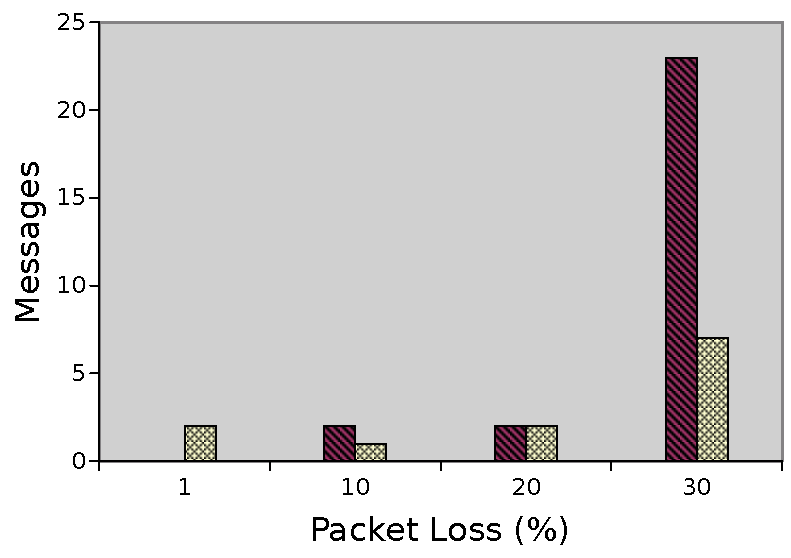
\includegraphics[width = \textwidth]{figures/hooo.pdf}
\caption{Host Out-of-Order Messages}
\label{fig:hooo}
\end{minipage}
\quad
\begin{minipage}[b]{0.48\linewidth}
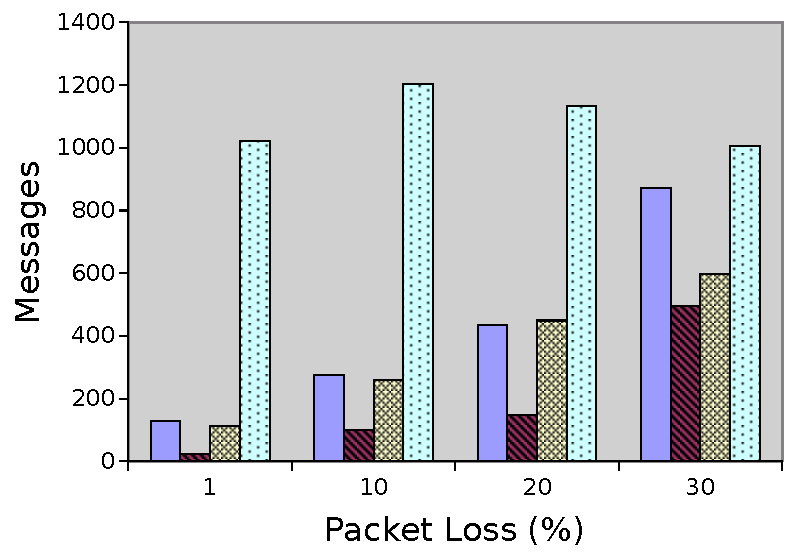
\includegraphics[width = \textwidth]{figures/gooo.pdf}
\caption{Global Out-of-Order Messages}
\label{fig:gooo}
\end{minipage}
\end{figure}

\begin{figure}[ht]
\centering
\begin{minipage}[b]{0.48\linewidth}
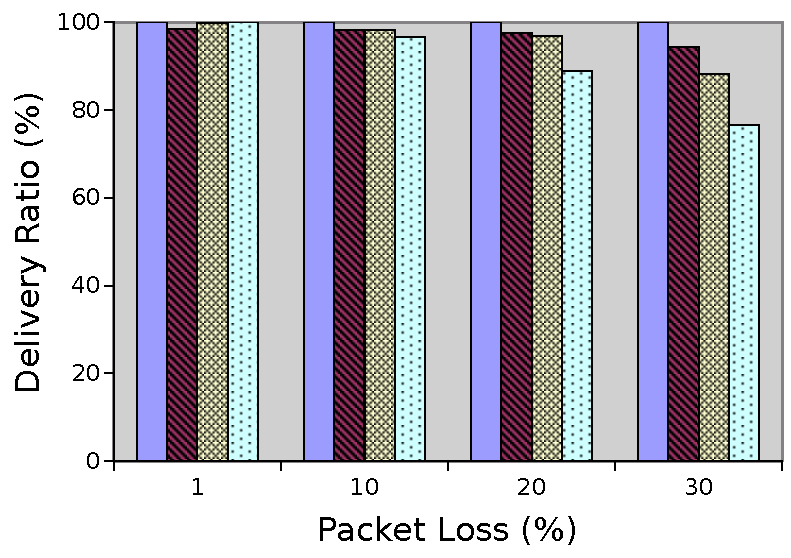
\includegraphics[width = \textwidth]{figures/delivery.pdf}
\caption{Delivery Rates}
\label{fig:delivery}
\end{minipage}
\quad
\begin{minipage}[b]{0.48\linewidth}
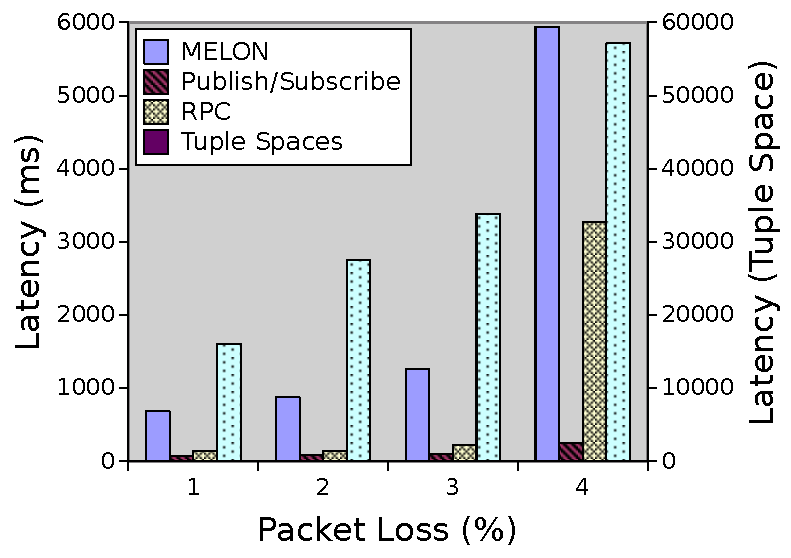
\includegraphics[width = \textwidth]{figures/latency.pdf}
\caption{Message Latency}
\label{fig:latency}
\end{minipage}
\end{figure}

In our experiments, messages from a single host were generally delivered in the order they were sent as shown in Figure \ref{fig:hooo}. For MELON and tuple spaces, no messages were delivered out of order. However, it should be noted that for tuple spaces this is an implementation accident, whereas in MELON it is guaranteed. In LighTS, tuples are sequentially stored locally in an array in the order they are output, then returned in that same order when they are matched. Tuple spaces in general do not return matched messages in any particular order.

In this application, RPC is used in an asynchronous manner since it is providing group communication. If one call is delayed, it is possible a subsequent call will complete before a prior one, which explains why RPC delivers a small number of messages out of order. Publish/subscribe is fully asynchronous and incoming publications can even be processed concurrently. However, even in the worst case publish/subscribe delivers 97.8\% of the messages from a host in the order they were sent. Unfortunately, like tuple spaces this is just the result of a single implementation and the RPC and publish/subscribe paradigms make no promises about the ordering of messages. 

Unlike per-host ordering, many messages were delivered out of order from a global perspective as can be seen in Figure \ref{fig:gooo}. This is entirely expected, since none of the paradigms provide a global ordering. Enforcing a global ordering in an unreliable network is not feasible, since nodes may become unavailable at anytime while continuing to output messages. However, the global ordering remains important for a shared whiteboard.

Our results show publish/subscribe performs the best for this metric. Indeed, ordering is largely dependent on deliveries completing quickly before later messages overtake them. As shown in Figure \ref{fig:latency}, publish/subscribe is an extremely quick method for delivering messages, so it excels in ordering as well. Conversely, tuple spaces fare the worst, delivering 67\% of messages out of order. Again, because tuple spaces provide no way of controlling which matches messages are returned or in what order, the whiteboard implementation must transfer large amounts of tuples in order to nondestructively read all matching messages. This is extremely slow, as reflected in Figure \ref{fig:latency}.

MELON and RPC perform about the same for global ordering, although MELON is more affected when the network conditions worsen. This is likely due to MELON's reliable message delivery (Figure \ref{fig:delivery}), since some messages may be delayed significantly by broken network routes or even network partitioning. In contrast, losing messages can improve ordering since a message not delivered cannot be out of order. Of the paradigms compared, MELON is the only one to demonstrate 100\% message delivery. Tuple spaces would also be expected to be reliable, but again in this application it is required to deliver large amounts of messages. Given that the median latency for tuple spaces reached a full minute, the experiment completed before some messages arrived.

While we have seen publish/subscribe have low delivery ratios in the past\cite{collins2010quantitative}, here it performs well in the lossy environment due to its quick delivery rates, but still dropped 1.4\% of messages when the network connectivity was good. RPC performs predictably, slowing losing more messages as the network degrades. Again, we are using group RPC, which means it does not know how many receives may be available and therefore does not retry to complete calls if a host cannot be reached for a period of time. Fully synchronous RPC it would block the process until the message is delivered. However, that would also delay deliveries considerably which is not acceptable for a whiteboard application.

Figure \ref{fig:latency} shows delivery latency. Since tuple spaces are so much slower, the results are correlated to the right-hand y-axis which is an order of magnitude higher. Publish/subscribe was extremely quick, which is typical since it requires no message confirmations nor active discovery of remote hosts. RPC was also quite fast until it was slowed down along with the other paradigms by the 30\% packet loss.

Logically, delivery rates and latency are directly related. With reliable delivery some messages may be very late, increasing overall latency. On the other hand, dropped messages do not count towards the latency metric, so a lossy communication paradigm can appear to be very fast. MELON errs on the side of reliability, and therefore is a bit slower as the network becomes less reliable and more delivery attempts are required. There is an additional trade-off that pull-based paradigms like MELON and tuple spaces must make, which is the frequency of the pull attempts. Publish/subscribe and RPC may send as soon as a message is ready, but MELON and tuple spaces must continually poll to receive messages. Faster polling results in faster message delivery, but higher overall network usage, collisions and resource monopolization.

\section{Related Work}\label{sec:relatedwork}

The concept of a distributed shared message store is based on the idea of tuple spaces introduced with the Linda\cite{linda} coordination language. Several projects have adapted tuple spaces to MANETs, including LIME\cite{lime}, TOTA\cite{tota}, TOTAM\cite{totam}, and EgoSpaces\cite{egospaces}, of which LIME is likely the most well-cited example.

The original version of LIME relies on explicit join and leave operations to federate distributed tuple spaces, which is at odds with the frequently unexpected disconnections in MANETs. \cite{limerevisted} discusses the difficulties LIME encounters when attempting to implement tuple space semantics, including situations that can lead to livelocks. LIME II\cite{lime2}, Limone\cite{limone}, and CoreLIME\cite{corelime} are projects intended to address the shortcomings in the original LIME.

Further surveys of middleware, languages, and communication paradigms for MANET development can be found in \cite{mine} and \cite{mwtrends}.

\section{Conclusions}\label{sec:conclusions}

Traditional distributed computing paradigms were not designed to operate in dynamic, self-organizing MANETs where disconnections and topology changes are frequent. In this paper we have qualitatively and quantitatively compared the MELON coordination language to traditional distributed computing paradigms. The results indicate the features of MELON are useful in a shared whiteboard application for MANETs while its performance was measured to be comparable to existing paradigms when operating in a MANET environment. This demonstrates MELON can serve as a practical approach to communication in MANET applications.

\bibliographystyle{unsrt}
\bibliography{refs}

\end{document}
